\subsubsection{Availability of Noise Samples within the Coherence Time}\label{subsubsec:disponibilidade-amostras}
All samples used in noise estimation must represent the same covariance matrix. Therefore, the sampling interval is limited by the variation in time and frequency of the channels that determine the interference. \textcolor{red}{These variations define the coherence block (Section~\ref{subsec:bloco-coerencia}). Thus, the estimate $\hat{\mathbf R}_{cc}$} is unique per PRB within each coherence time.


\textcolor{blue}{The Demodulation Reference Signal (DM-RS) in 5G NR is the reference signal (pilot) transmitted by the UE to allow the receiver to estimate channel conditions.} The DM-RS is transmitted alongside the PUSCH (Section~\ref{subsec:simbolos}) within the same PRBs. The double-symbol DM-RS occupies two consecutive OFDM symbols at each position within the slot and allows for the differentiation of up to 12 UEs \cite{3gpp-ts38211}.
% FONTE: TS 38.211 Sec. 6.4.1.1.3, Tabs. 6.4.1.1.3-2, 6.4.1.1.3-4 e 6.4.1.1.3-5.

\textcolor{red}{The receiver obtains the} noise samples from the REs occupied by the DM-RS. \textcolor{red}{Assim, só há amostras nos slots em que os UEs alvo transmitem o PUSCH.} The number of samples therefore depends on how many DM-RS REs are present within the interval over which the covariance remains constant. \textcolor{blue}{The double-symbol DM-RS occupies 4 OFDM symbols, with a maximum of two positions per slot \cite{3gpp-ts38211}.} \textcolor{red}{Thus,} each PRB \textcolor{red}{has at most} 4 $\times$ 12 = 48 DM-RS REs per slot. Figure~\ref{fig:prb-dmrs} illustrates these REs within a PRB.

\definecolor{dmrsfill}{HTML}{CDE2FB}
\definecolor{winblue}{HTML}{0D366B}
\definecolor{inksec}{HTML}{52514E}
\begin{figure}[htbp]
\caption[Resource elements of one PRB in one slot, with the DM-RS symbols.]{Resource elements of one PRB in one slot, with the DM-RS symbols. Double-symbol DM-RS, mapping type~A, symbols 2, 3, 10 and 11.}
\label{fig:prb-dmrs}
\vspace{4pt}
\centering
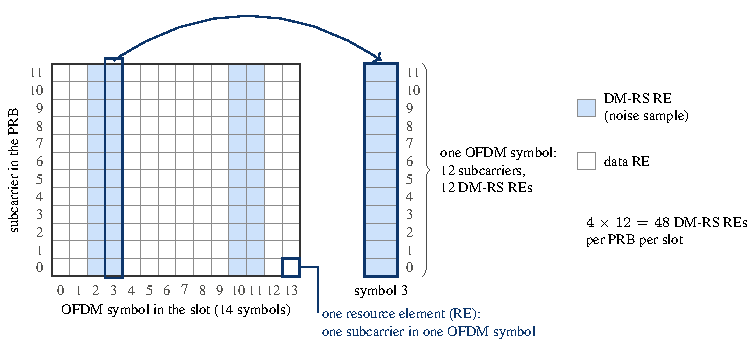
\includegraphics{Images/FLUXO/prb_dmrs.pdf}
\vspace{4pt}
\legend{Source: the author, with the DM-RS positions of \citesp{3gpp-ts38211}.}
\end{figure}


\textcolor{red}{Since the samples must fall within the same interval of duration $T_c$ as the data symbol,} the number of available samples may vary from one data symbol to another. \textcolor{blue}{The number of samples for a given symbol corresponds to the maximum count of DM-RS REs found within an interval of duration $T_c$ that encompasses that symbol.} The number of samples available for all symbols in the slot is the smallest of these values. Figure~\ref{fig:dmrs-n} shows an example with the DM-RS located at symbols 2, 3, 10, and 11 of each slot. \textcolor{red}{Symbols 5 through 8 are the worst case under the TDLB100-400 condition}, with 24 samples. Therefore, the number of samples available for all symbols is 24. Table~\ref{tab:n-maximo} presents this value for each test condition.

\begin{table}[htbp]
\caption[Number of DM-RS REs per PRB available to every data symbol of the slot, in each test condition.]{Number of DM-RS REs per PRB available to every data symbol of the slot, in each test condition. Double-symbol DM-RS in symbols 2, 3, 10 and 11, with every slot carrying PUSCH.}
\label{tab:n-maximo}
\vspace{4pt}
\centering
\footnotesize
\renewcommand{\arraystretch}{1.2}
\setlength{\aboverulesep}{0pt}
\setlength{\belowrulesep}{0pt}
\begin{tabular}{|c|c|c|c|c|}
\toprule
\multirow{2}{*}{\textbf{Test condition}} & \textbf{Frequency} & \multirow{2}{*}{{\boldmath $T_c$} \textbf{(ms)}} & \textbf{OFDM symbols} & \textbf{DM-RS REs} \\
 & \textbf{range} & & \textbf{in} {\boldmath $T_c$} & \textbf{available} \\
\midrule
TDLA30-5    & \multirow{2}{*}{FR1} & 25.0000 & 700 & 2400 \\
TDLA30-10   &                      & 12.5000 & 350 & 1200 \\
\cline{2-2}
TDLA30-75   & \multirow{2}{*}{FR2} & 1.6667  & 186 & 648 \\
TDLA30-300  &                      & 0.4167  & 46  & 168 \\
\cline{2-2}
TDLC300-100 & \multirow{4}{*}{FR1} & 1.2500  & 35  & 132 \\
TDLB100-400 &                      & 0.3125  & 8   & 24 \\
HST350      &                      & 0.0536  & \multirow{2}{*}{1} & \multirow{2}{*}{0} \\
HST500      &                      & 0.0375  &     &  \\
\bottomrule
\end{tabular}
\vspace{4pt}
\legend{Source: the author, from \citesp{3gpp-ts38104}; \citesp{3gpp-ts38211}; \citesp{tse-viswanath}.}
\end{table}

\textcolor{red}{The interval with the most DM-RS REs for a data symbol} may include DM-RS that arrive after that symbol. In Figure~\ref{fig:dmrs-n}(b), \textcolor{red}{this interval for} symbol 13 goes up to symbol 3 of the next slot. \textcolor{blue}{The receiver needs to store symbol 13 for 4 more symbols to use these samples.}
% FONTE: contagens em Python (DM-RS em {2,3,10,11}, slots contínuos, L = 8).
\definecolor{dmrsfill}{HTML}{CDE2FB}
\definecolor{winblue}{HTML}{0D366B}
\definecolor{inksec}{HTML}{52514E}
\begin{figure}[htbp]
\caption[Intervals of duration $T_c$ that contain a data symbol, and their DM-RS REs per PRB, in the TDLB100-400 condition.]{Intervals of duration $T_c$ that contain a data symbol, and their DM-RS REs per PRB, in the TDLB100-400 condition. Double-symbol DM-RS, mapping type~A, symbols 2, 3, 10 and 11; continuous uplink. In (a) and (b), each bar is one position of an interval of duration $T_c$ that contains the marked symbol. Symbol 6 is the worst case of the slot, and symbol 13 is a best case.}
\label{fig:dmrs-n}
\vspace{4pt}
\centering
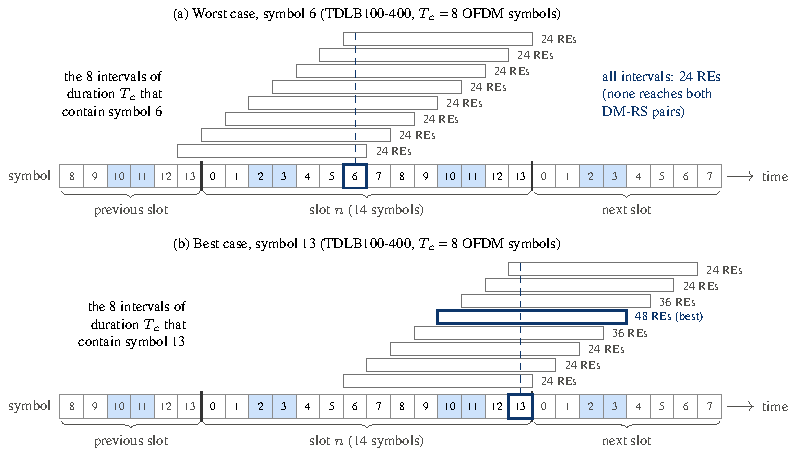
\includegraphics{Images/FLUXO/dmrs_n.pdf}
\vspace{4pt}
\legend{Source: the author, with the DM-RS positions of \citesp{3gpp-ts38211}.}
\end{figure}

